\chapter{Entwickelte Methode}
\chaptermark{Entwickelte Methode}  % short form for headlines on pages
\label{ch:EntwickelteMethode}

Dieses Kapitel beschreibt zunächst die nachvollziehbare Aufbereitung der
Rohdaten und anschließend die Anomalieerkennung anhand von Prognosefehlern.
Methodische Entscheidungen werden von den später berichteten
Ergebnissen getrennt dargestellt.

\section{Datengrundlage}
\label{sec:Methode_Datengrundlage}

Die Rohdaten liegen in Form einer JSON-Datei mit 17.578 Einzelmessungen vor. Jede
Messung gehört zu einem von 30 Sensorstandorten in der Innenstadt und im
Kurpark von Bad Nauheim und enthält neben dem Zeitstempel die Anzahl der
erfassten Passanten (\texttt{visitors}) sowie deren mittlere Verweildauer
(\texttt{avgDuration}). Der globale Erfassungszeitraum reicht vom 30.~Juni bis
zum 13.~Juli 2025 und umfasst 335 Stunden. Sensorindividuelle Soll-Laufzeiten
liegen nicht vor. Deshalb wird konservativ nur der Zeitraum zwischen erster und
letzter beobachteter Messung als Laufzeit verwendet. Dadurch entstehen 9.460
aktive Sensorstunden; 590 Kombinationen des globalen Rasters werden vorläufig
nicht als Messlücke behandelt. Diese Annahme verhindert künstliche Randwerte,
kann einen frühen oder späten Ausfall aber fälschlich als Inaktivität deuten.
Beobachtete und noch zu bestätigende Grenzen stehen deshalb getrennt in
\texttt{data/sensor\_activity\_periods.csv}.

\section{Datenqualität}
\label{sec:Methode_Datenqualitaet}

Bei der Sichtung der Rohdaten sind zwei Probleme aufgefallen, die vor dem
Training behandelt werden müssen.

\textbf{Mehrfachmessungen:} Für 4.770 Kombinationen aus Sensor und Stunde
enthält der Datensatz mehrere Einträge, in der Spitze zehn Messungen für
dieselbe Stunde (Abbildung~\ref{fig:preproc_mehrfach}). Die Werte dieser
Einträge weichen teilweise voneinander ab, es handelt sich also nicht um
exakte Kopien. Ohne Bereinigung gingen diese Stunden mehrfach und mit
widersprüchlichen Werten in das Training ein.

\begin{figure}[htb]
  \centering
  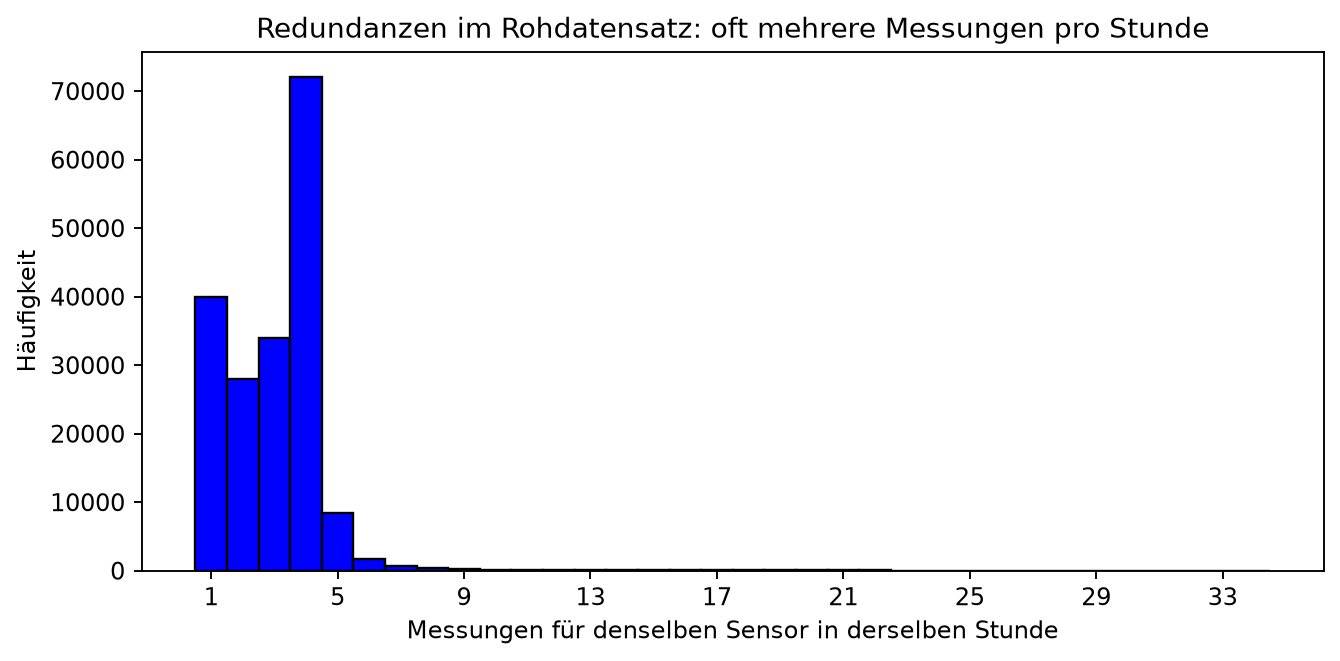
\includegraphics[width=0.75\textwidth]{Figures/preproc_mehrfachmessungen.png}
  \caption{Häufigkeit von Mehrfachmessungen im Rohdatensatz. Für viele
    Stunden liegen zwei bis vier, vereinzelt bis zu zehn Einträge desselben
    Sensors vor.}
  \label{fig:preproc_mehrfach}
\end{figure}

\textbf{Messlücken:} Nach der Zusammenfassung und Qualitätsprüfung liegen
6.814 gültig gemessene Sensorstunden vor. Innerhalb der 9.460 aktiven
Sensorstunden fehlen damit 2.646 Werte, entsprechend 28{,}0~\%. Sie bilden 830
zusammenhängende Lücken. Davon umfassen 641 höchstens zwei Stunden; die längste
Lücke innerhalb einer aktiven Sensorperiode dauert 18 Stunden
(Abbildung~\ref{fig:preproc_lueckenlaengen}). In 63 Stunden liegt von keinem
der zu diesem Zeitpunkt aktiven Sensoren eine Messung vor. Dies deutet auf
gemeinsame Ausfälle der Übertragungsinfrastruktur hin. Die Sensoren
Kurpark--Eingang Ludwigstraße und Friedrichstraße~1 besitzen mit 36
beziehungsweise 59 Stunden lediglich kurze aktive Erfassungszeiträume. Zeiten
nach ihrem letzten Messwert werden nicht künstlich ergänzt. Ob ihr früher
Abbruch eine geplante Deaktivierung oder einen Ausfall darstellt, muss durch
Betreiberinformationen geklärt werden.

Am 5.~Juli 2025 um 08:00~Uhr UTC meldeten alle 28 zu diesem Zeitpunkt aktiven
Sensoren gleichzeitig exakt null Besucher und null Verweildauer. Dieses
stadtweite identische Muster wird als gemeinsamer Erfassungs- oder
Übertragungsfehler behandelt. Die 28 Werte bleiben über die Quellenanzahl
nachvollziehbar, gelten aber für Modellierung und Evaluation als fehlend.

\begin{figure}[htb]
  \centering
  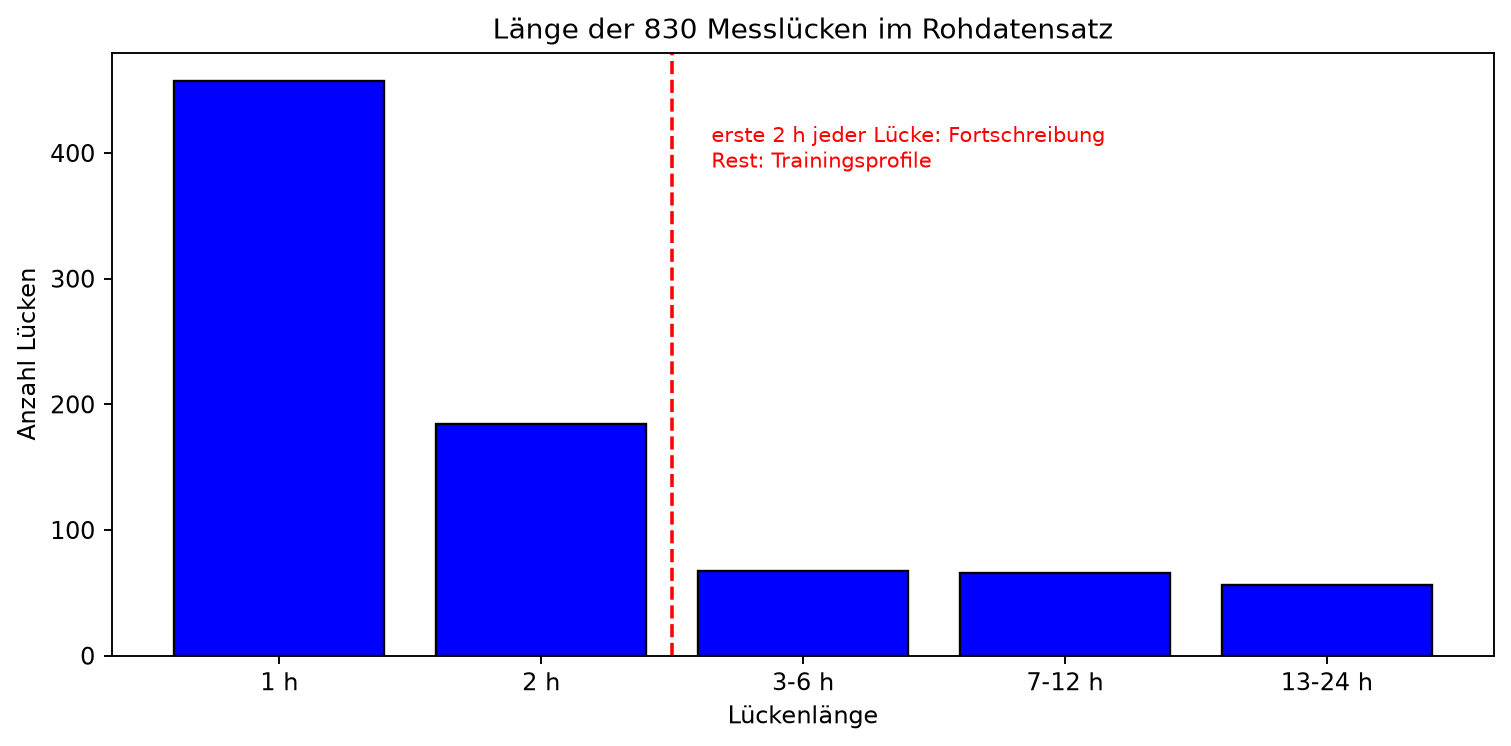
\includegraphics[width=0.8\textwidth]{Figures/preproc_lueckenlaengen.png}
  \caption{Längenverteilung der 830 Messlücken innerhalb der angenommenen
    Sensorperioden. 641 Lücken umfassen höchstens zwei Stunden.}
  \label{fig:preproc_lueckenlaengen}
\end{figure}

\section{Bereinigung der Mehrfachmessungen}
\label{sec:Methode_Dedup}

Alle Einträge derselben Kombination aus Sensor und Stunde werden zu einem
Messpunkt zusammengefasst. Für die Passantenzahl und die Verweildauer wird
jeweils der arithmetische Mittelwert gebildet. Dadurch verbleiben zunächst
6.842 eindeutige Stundenwerte. Nach Ausschluss der 28 gemeinsamen
Nullmeldungen gelten 6.814 davon als gemessen. Nach Abschluss der Imputation
wird die Passantenzahl auf ganze Personen und die Verweildauer auf zwei
Dezimalstellen gerundet.

\section{Behandlung der Messlücken}
\label{sec:Methode_Imputation}

Die für das Training verwendeten Zeitfenster setzen zusammenhängende
Stundenreihen voraus. Eine Lücke innerhalb eines Fensters würde andernfalls
unbemerkt Werte aus weit auseinanderliegenden Zeiträumen kombinieren. Die
Lücken werden deshalb vor dem Training aufgefüllt, und zwar für jeden Sensor
getrennt, damit jeder Standort sein individuelles Niveau und Tagesprofil
behält. Die zentrale Datenaufbereitung verwendet keine lineare Interpolation.
Sämtliche Profile werden ausschließlich aus ursprünglich gemessenen Werten vor dem
8.~Juli 2025, 00:00~Uhr UTC, geschätzt; Validierungs-, Kalibrierungs- und
Testwerte gehen damit nicht in die Profilbildung ein. Wochentag und Stunde
werden in der lokalen Zeitzone \texttt{Europe/Berlin} bestimmt. Das Verfahren
arbeitet in vier aufeinanderfolgenden Stufen.

\textbf{Stufe 1, vergangenheitsbasierte Fortschreibung:} Für die ersten zwei
Stunden jeder Lücke wird der letzte zuvor gemessene Wert desselben Sensors
übernommen. Mit $t^{-}$ als Zeitpunkt der letzten Messung gilt
\begin{equation}
  \hat{x}_t=x_{t^{-}}, \qquad 0<t-t^{-}\leq 2\ \text{Stunden}.
\end{equation}
Diese Regel gilt auch für die ersten beiden Positionen einer längeren Lücke.
Sie benötigt keinen nachfolgenden Messwert und verhindert dadurch, dass ein
späteres Prognoseziel in einen früheren Modellkontext zurückgespiegelt wird.
Der Preis ist eine kurzfristig konstante Fortsetzung; die Regel stellt daher
einen transparenten Kompromiss und kein allgemein optimales
Imputationsverfahren dar. Auf diese Weise werden 1.203 Sensorstunden ergänzt.

\textbf{Stufe 2, Wochentag-Stunden-Profil:} Für die verbleibenden Lücken wird
der Mittelwert desselben Sensors am gleichen lokalen Wochentag und zur gleichen
lokalen Stunde aus gemessenen Trainingswerten eingesetzt. Historische
Zeitprofile erhalten tages- und wochenzeitabhängige Strukturen und werden auch
für fehlende Verkehrszähldaten untersucht \cite{sun_traffic_2022}. Diese Stufe
füllt 1.298 Sensorstunden.

\textbf{Stufe 3, Stundenprofil:} Existiert für eine Kombination aus Wochentag
und Stunde keine Trainingsreferenz, wird der Mittelwert des Sensors zur
gleichen lokalen Uhrzeit über alle Trainingstage verwendet. Dies betrifft 140
Sensorstunden.

\textbf{Stufe 4, Sensormittel:} Fehlt auch für die betreffende Uhrzeit eine
Referenz, wird der Mittelwert sämtlicher gemessener Trainingswerte dieses
Sensors eingesetzt. Diese Rückfallstufe betrifft fünf Sensorstunden. Damit
werden alle 2.646 Lücken innerhalb der angenommenen Sensorperioden geschlossen;
Zeiten vor der ersten und nach der letzten Messung eines Sensors bleiben
außerhalb des Datensatzes.

\begin{figure}[htb]
  \centering
  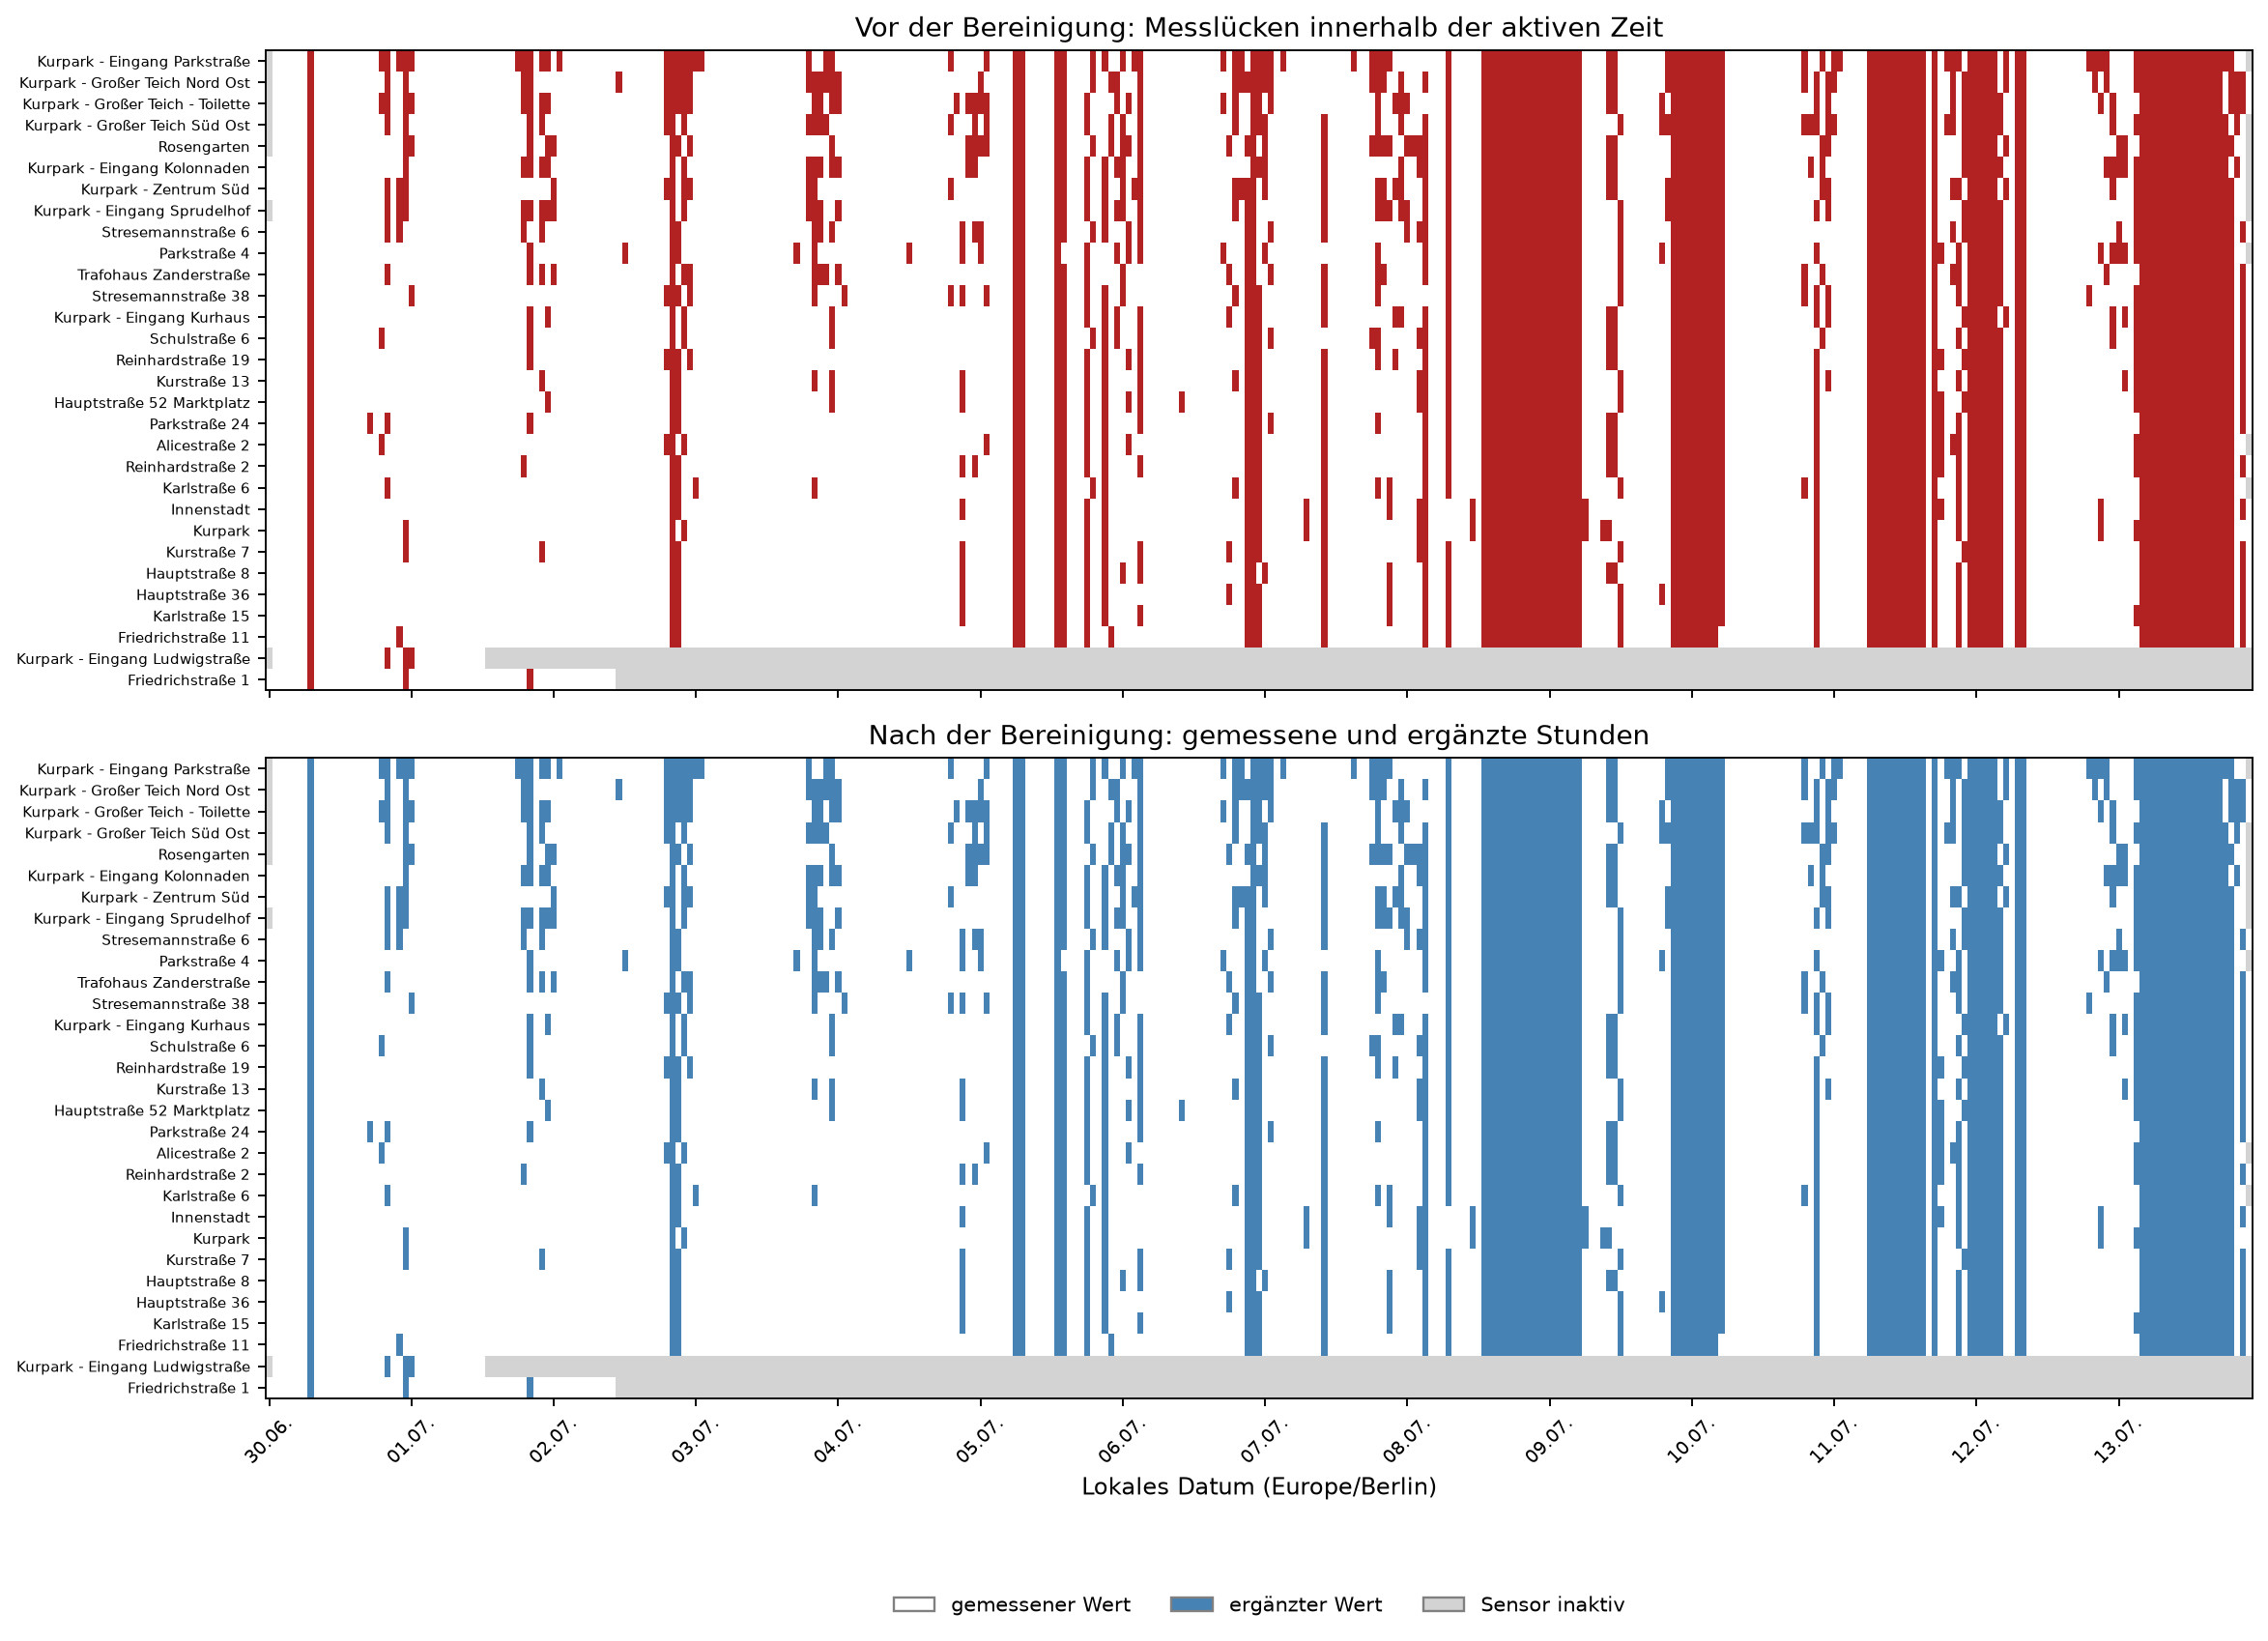
\includegraphics[width=\textwidth]{Figures/preproc_luecken_heatmap.png}
  \caption{Messstatus vor der Bereinigung (oben) und danach (unten). Rot zeigt
    Lücken innerhalb der aktiven Sensorzeit, Blau ergänzte Werte und Grau
    Zeiträume, in denen der betreffende Sensor nicht aktiv war. Eigene
    Darstellung.}
  \label{fig:preproc_heatmap}
\end{figure}

Der untere Teil von Abbildung~\ref{fig:preproc_heatmap} kennzeichnet die
ergänzten Stunden. Abbildung~\ref{fig:preproc_beispiele} stellt eine typische
Reihe und den Sensor mit der kürzesten aktiven Erfassungszeit gegenüber. Sie
zeigt zugleich, dass die Reihe nach dem Ende des Sensors nicht künstlich
fortgeschrieben wird. Abbildung~\ref{fig:preproc_anteil} fasst den ergänzten
Anteil innerhalb der aktiven Zeit jedes Sensors zusammen.

\begin{figure}[htb]
  \centering
  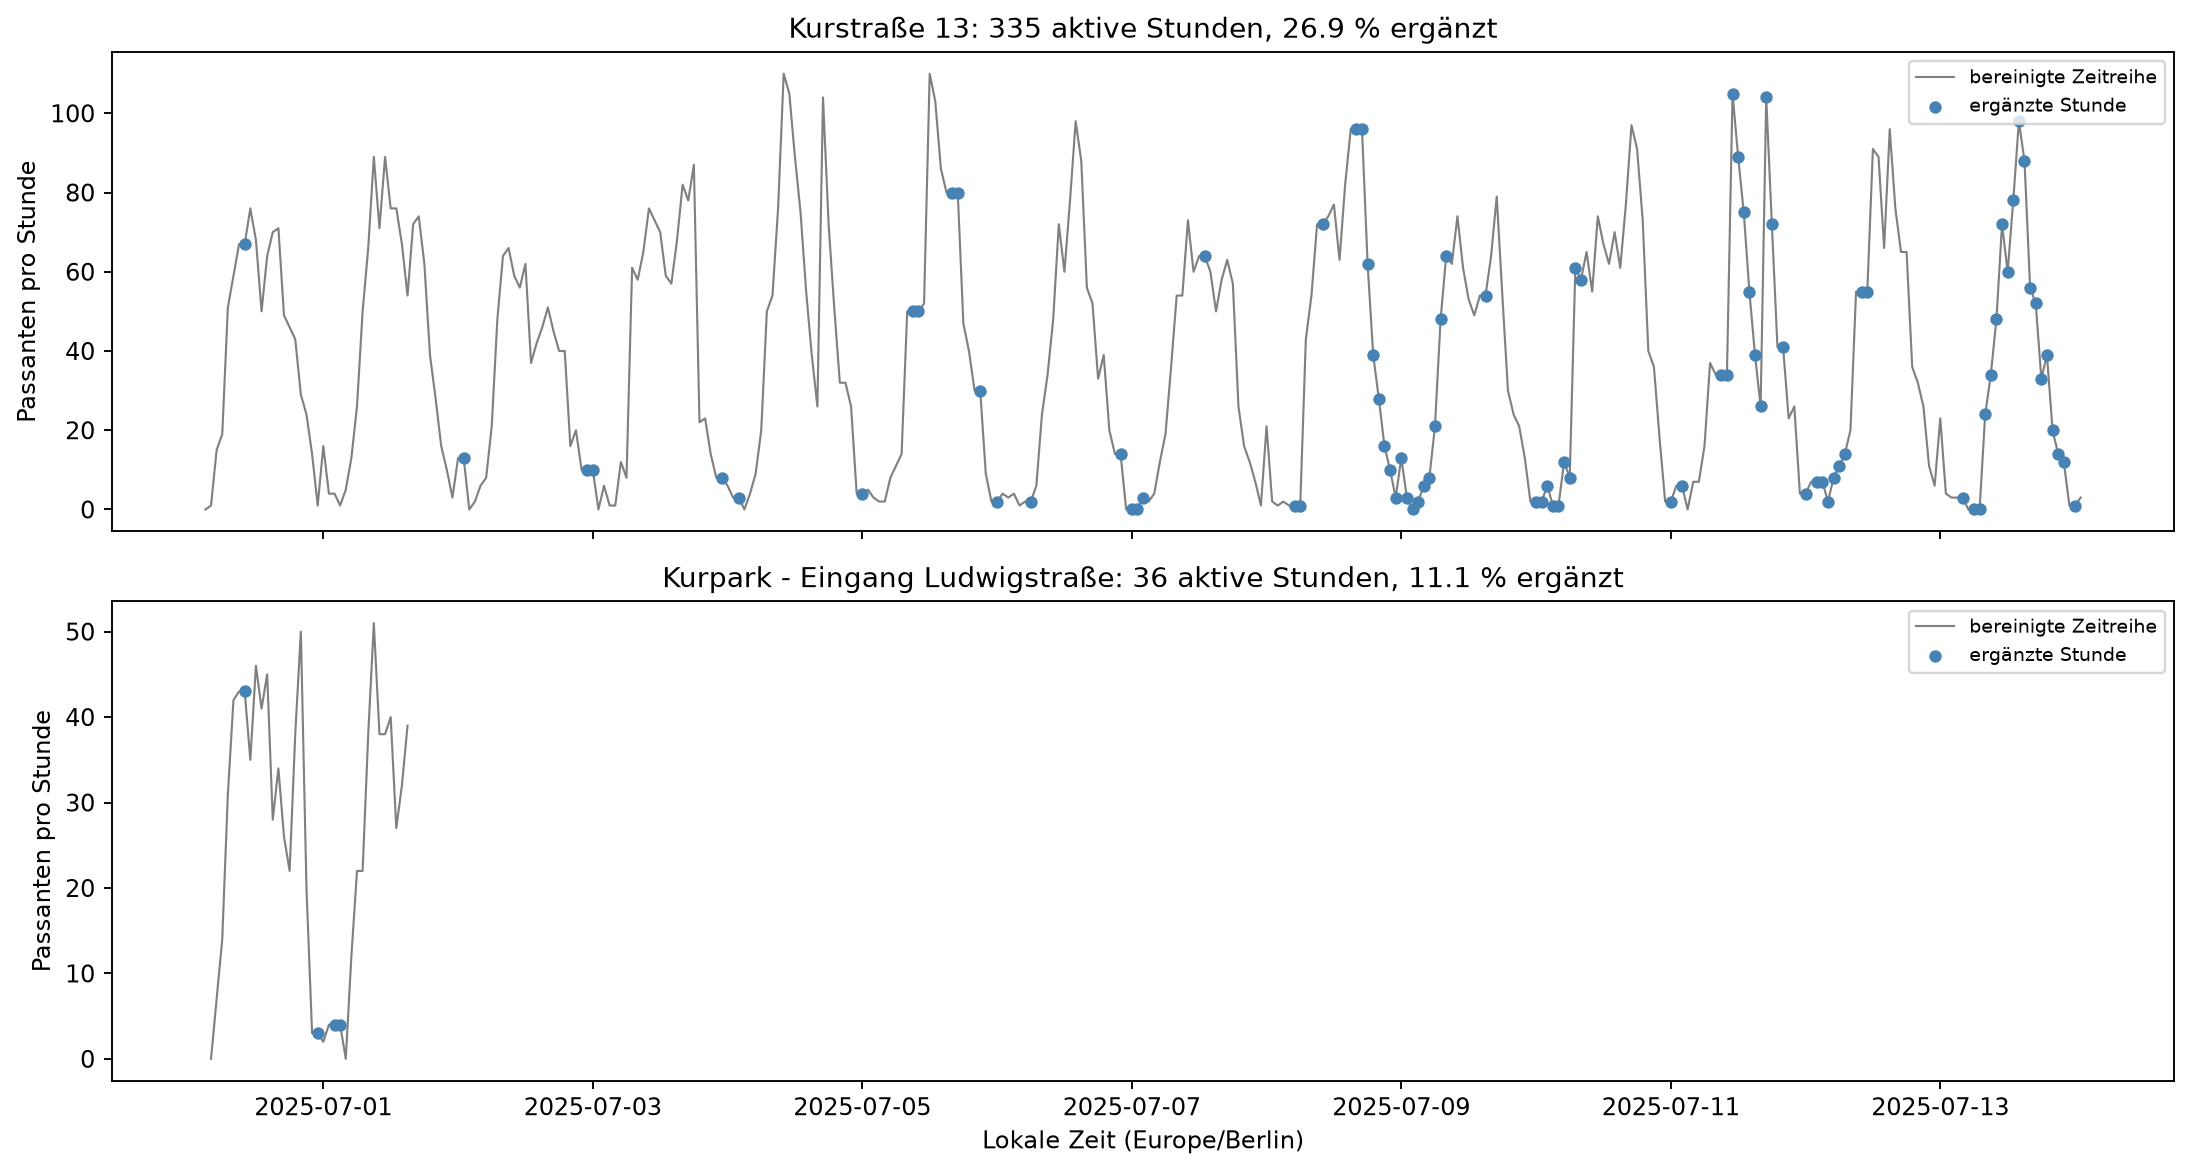
\includegraphics[width=\textwidth]{Figures/preproc_beispielreihen.png}
  \caption{Bereinigte Zeitreihen eines typischen Sensors (oben) und des
    Sensors mit der kürzesten aktiven Erfassungszeit (unten). Markierte Punkte
    sind ergänzte Stunden. Eigene Darstellung.}
  \label{fig:preproc_beispiele}
\end{figure}

\begin{figure}[htb]
  \centering
  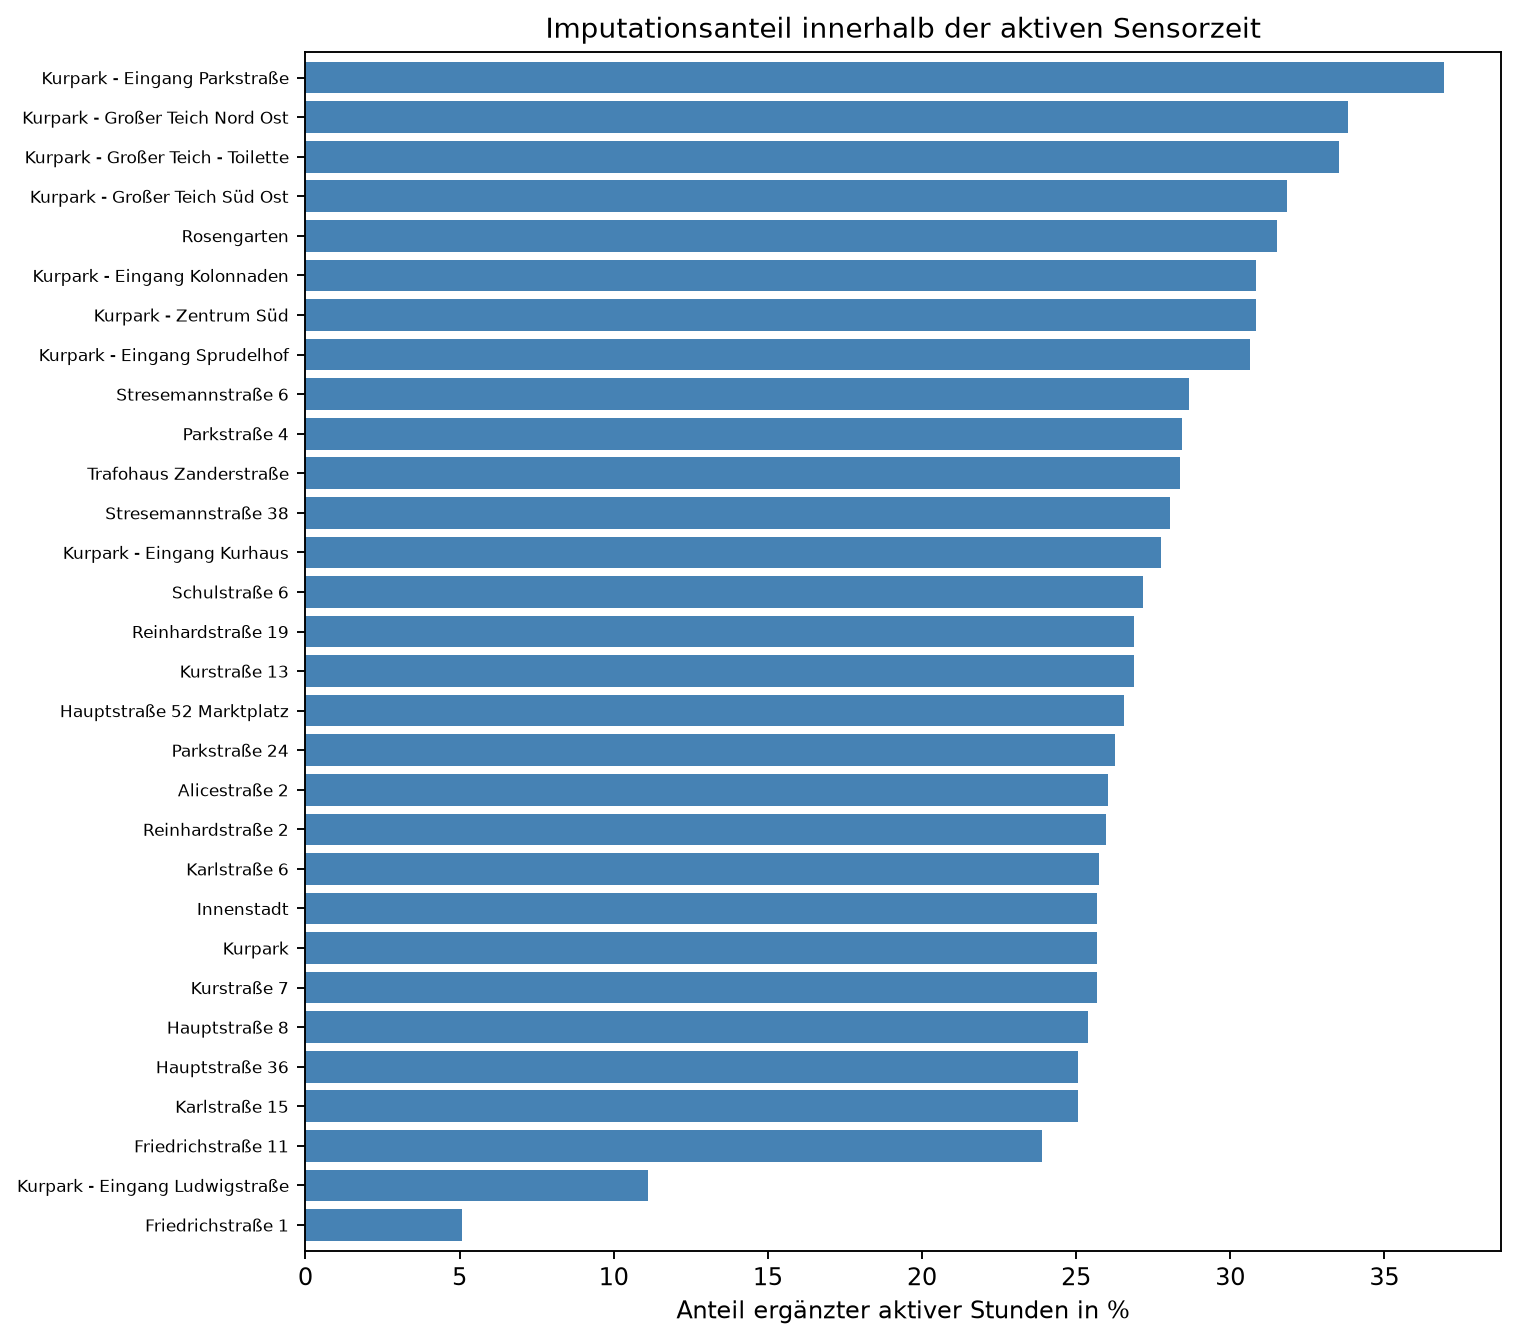
\includegraphics[width=0.85\textwidth]{Figures/preproc_imputationsanteil.png}
  \caption{Anteil ergänzter Stunden innerhalb der aktiven Zeit jedes Sensors.
    Eigene Darstellung.}
  \label{fig:preproc_anteil}
\end{figure}

\section[Kritische Betrachtung]{Kritische Betrachtung der Bereinigung}
\label{sec:Methode_Kritik}

Jede Imputation verändert die Daten. Mittelwertbasierte Verfahren können den
Verlauf glätten und die Varianz verringern
\cite{zhang_survey_2024,shafique_hourly_2022}. Im vorliegenden Datensatz ändert
sich der Mittelwert der Passantenzahl je Sensor um höchstens 10{,}29~\%. Die
kleinste Korrelation zwischen dem ausschließlich aus gemessenen Werten und dem
aus allen bereinigten Werten gebildeten stündlichen Tagesprofil beträgt
0{,}9843. Diese Kennzahlen prüfen Niveau und Profil, ersetzen aber keine
Fehleranalyse gegen unbekannte wahre Werte in den Lücken.

Gemessene Werte werden nicht zusätzlich geglättet. Eine Glättung könnte
kurzzeitige echte Abweichungen abschwächen und damit gerade das gesuchte Signal
entfernen. Die Stabilisierung beschränkt sich deshalb auf Aggregation,
Transformation und Skalierung; die Folgen der Imputation werden separat durch
künstliches Entfernen bekannter Messwerte geprüft.

Die zweistündige Fortschreibung verwendet zu jedem Zeitpunkt nur die
Vergangenheit. Die statistischen Profile dürfen dagegen innerhalb des
Trainingsabschnitts auch chronologisch spätere Trainingsmessungen enthalten.
Für die Aufbereitung werden keine Validierungs- oder Testwerte verwendet.
Innerhalb des Trainingsabschnitts können jedoch spätere Trainingsmessungen in
die Profile einfließen; die Ergänzung ist dort also nicht zu jedem Zeitpunkt
ausschließlich vergangenheitsbasiert.

Ein zweiter Aspekt betrifft die Anomalieerkennung selbst. Ergänzte Stunden
wirken per Konstruktion unauffällig, ein tatsächlicher Sensorausfall stellt
jedoch selbst ein meldenswertes Ereignis dar. Das Fehlen von Werten folgt
hier zudem eigenen, teils blockweisen Mustern und trägt damit selbst
Information \cite{zhang_survey_2024}. Das Feld \texttt{is\_imputed} hält für
jede Stunde fest, ob sie gemessen oder ergänzt wurde. Das Prognosemodell
verwendet ergänzte Werte weiterhin als Kontext eines 24-Stunden-Fensters, überspringt
jedoch Fenster mit einem ergänzten Zielwert beim Training, bei der Bestimmung
des Schwellenwerts und bei der Testauswertung. Die beiden besonders kurzen
Sensorreihen werden wegen ihrer geringen aktiven Länge nicht verwendet.

\section[Prognosemodell]{Anomalieerkennung anhand von Prognosefehlern}
\label{sec:Methode_Forecaster}

\subsection{Lernaufgabe und Eingaberepräsentation}

Das Prognosemodell lernt selbstüberwacht, aus den jeweils vorhergehenden 24
Stunden die nächste Stunde vorherzusagen. Die nachgelagerte Anomalieentscheidung ist
unüberwacht, da weder das Modelltraining noch die Kalibrierung reale
Anomalieklassen verwenden. Ein einziges gemeinsames Modell wird über 28 Sensoren
trainiert. Zwei Sensoren werden ausgeschlossen, weil vor dem Ende des
Trainingsabschnitts weniger als 72 gemessene Zielstunden vorliegen.

Beide Zielgrößen werden zunächst mit $\log(1+x)$ transformiert. Danach erfolgt
eine globale Standardisierung je Merkmal~$f$:
\begin{equation}
  z_{t,f}=\frac{\log(1+x_{t,f})-\mu_f}{\sigma_f}.
\end{equation}
Mittelwert und Standardabweichung werden ausschließlich aus gemessenen
Trainingswerten bestimmt. Jedes Zeitfenster besitzt genau drei Kanäle:
\texttt{visitors}, \texttt{avgDuration} und eine Maske, die gemessene von
imputierten Kontextwerten unterscheidet. Die Ausgabe enthält zwei
Vorhersagewerte. Zusätzliche Kalendermerkmale und eine vom Netz gelernte
Sensorcodierung werden
wegen der kurzen Einzelreihen und der gewünschten Einfachheit nicht verwendet.

\subsection{Modellarchitektur und Training}

Das LSTM \cite{hochreiter1997long} folgt einer einfachen
\texttt{Sequential}-Struktur:
\begin{equation}
  \operatorname{Input}(24,3) \rightarrow \operatorname{LSTM}(32)
  \rightarrow \operatorname{Dropout}(0{,}1)
  \rightarrow \operatorname{Dense}(16,\mathrm{ReLU})
  \rightarrow \operatorname{Dense}(2).
\end{equation}
Das Modell besitzt 5.170 Parameter. Der lineare \texttt{Dense(2)}-Ausgang gibt
die zwei Zielgrößen aus. \texttt{LSTM(32)} und \texttt{Dense(16)} halten das
Netz klein; Dropout wirkt einer zu starken Anpassung an die kurzen
Trainingsreihen entgegen \cite{srivastava2014dropout}.

Trainiert wird mit Adam, MSE und Batchgröße 128 für 54 Epochen auf Training plus
Validierung. Die Daten für Schwellenbestimmung und Test werden dabei nicht zum
Trainieren verwendet.

\subsection{Anomaliewert aus dem Prognosefehler}

Der absolute Prognosefehler jedes Merkmals wird durch seinen medianen absoluten
Fehler im Kalibrierungsabschnitt geteilt:
\begin{equation}
 r_{t,f}=\frac{|z_{t,f}-\hat z_{t,f}|}
 {\max\{\operatorname{Median}_{\mathrm{Kal}}(|z_f-\hat z_f|),0{,}05\}},
\end{equation}
Die zwei Fehlerverteilungen sind unterschiedlich breit. Deshalb erhält jedes
Merkmal eine eigene Grenze
\begin{equation}
 \tau_f=Q_{0{,}99}^{\mathrm{Kal}}(r_f), \qquad
 s_t=\max_f\frac{r_{t,f}}{\tau_f}, \qquad
 A_t=\mathbf{1}(s_t>1).
\end{equation}
Ein Alarm entsteht, sobald \texttt{visitors} oder \texttt{avgDuration} seine
eigene 99-\%-Grenze überschreitet. Der Gesamtwert $s_t$ hat für beide
Messgrößen dieselbe Alarmgrenze eins. Die Grenze wird nur aus den vorhandenen
Kalibrierungsfehlern geschätzt; eine feste spätere Fehlalarmrate ist dadurch
nicht garantiert.

\subsection{Umgang mit imputierten Zielwerten}

Imputierte Werte dürfen als markierter Kontext in ein Zeitfenster eingehen,
werden aber nicht als Ziel für Training, Modellauswahl, Kalibrierung oder
Prognosekennzahlen verwendet. Eine fehlende Originalmessung wird unabhängig von
der Prognose als Datenqualitätsereignis ausgegeben. Dadurch wird ein aus einem
Zeitprofil erzeugter Ersatzwert weder als reguläre Beobachtung noch als
bestätigte Verhaltensanomalie fehlinterpretiert.

\subsection{Vergleichsverfahren}

Zur Einordnung werden drei einfache Verfahren ohne neuronales Netz verwendet:
der Wert 24 Stunden zuvor, ein Sensor-Stundenmittel ausschließlich aus
gemessenen Trainingswerten und der Median der vorhergehenden 24 Stunden. Alle
vier Verfahren erhalten dieselben Testzeitpunkte. Damit zeigt der Vergleich,
ob das LSTM gegenüber leicht erklärbaren Regeln einen Mehrwert liefert.

